
\label{sec:discretization}

\begin{figure}[!ht]
  \centering
  
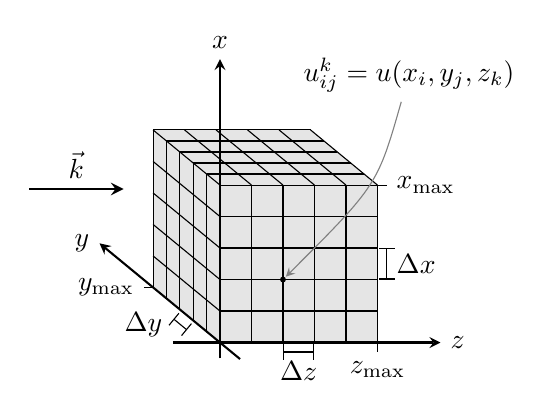
\begin{tikzpicture}[x={(0.0cm,0.4cm)},y={(-0.17cm,0.14cm)},z={(0.4cm,0.0cm)},>=stealth]

% box fill
\def\sidelength{5}

\fill[black!10] (xyz cs:x=0) -- (xyz cs:y=\sidelength) -- (xyz cs:x=\sidelength,y=\sidelength)  -- (xyz cs:x=\sidelength,y=\sidelength,z=\sidelength)  -- (xyz cs:x=\sidelength,z=\sidelength) -- (xyz cs:z=\sidelength);

% box grid
\foreach \coo in {1,2,...,\sidelength}{
  \draw (xyz cs:x=\coo) -- (xyz cs:z=\sidelength,x=\coo);
  \draw (xyz cs:x=\coo) -- (xyz cs:y=\sidelength,x=\coo);

  \draw (xyz cs:y=\coo) -- (xyz cs:x=\sidelength,y=\coo);
  \draw (xyz cs:y=\coo,x=\sidelength) -- (xyz cs:x=\sidelength,z=\sidelength,y=\coo);

  \draw (xyz cs:z=\coo) -- (xyz cs:x=\sidelength,z=\coo);
  \draw (xyz cs:z=\coo,x=\sidelength) -- (xyz cs:x=\sidelength,y=\sidelength,z=\coo);
}

% axes
\draw[line width=0.75pt,->] (xyz cs:x=-0.5) -- (xyz cs:x={\sidelength+4}) node[above] {$x$} ;
\draw[line width=0.75pt,->] (xyz cs:y=-1.5) -- (xyz cs:y={\sidelength+4}) node[left] {$y$};
\draw[line width=0.75pt,->] (xyz cs:z=-1.5) -- (xyz cs:z={\sidelength+2}) node[right] {$z$};

\draw [arrows={|-|}] (xyz cs:z={\sidelength+0.3pt},x=2) -- node[right] {$\Delta x$} (xyz cs:z={\sidelength+0.3pt},x=3);
\draw [|-|] (xyz cs:x=-0.3pt,y=2,z=-0.2pt) -- node[left = 3pt] {$\Delta y$} (xyz cs:x=-0.3pt,y=3,z=-0.2pt);
\draw [|-|] (xyz cs:x=-0.3pt,z=2) -- node[below] {$\Delta z$} (xyz cs:x=-0.3pt,z=3);

\draw (xyz cs:y=\sidelength) -- (xyz cs:y=\sidelength,z=-0.3pt) node[left] {$y_\mathrm{max}$};
\draw (xyz cs:x=\sidelength,z=\sidelength) -- (xyz cs:x=\sidelength,z={\sidelength+0.3pt}) node[right] {$x_\mathrm{max}$};
\draw (xyz cs:z=\sidelength) -- (xyz cs:x=-0.3pt,z={\sidelength}) node[below] {$z_\mathrm{max}$};

\draw [line width=1pt,->] (xyz cs:x=4,y=2.5,z=-5) -- node[above] {$\vec{k}$} (xyz cs:x=4,y=2.5,z=-2) ; 

\node[fill,circle,inner sep=0.75pt] at (2,0,2) {};

\node[align=center] at (8.5,0,6) (ori) {$u_{ij}^k = u(x_i,y_j,z_k)$};
\draw[->,color=gray,shorten >=1.5pt] (ori) .. controls (5,0,5)  .. (2,0,2);

\end{tikzpicture}

  \caption{We discretize the complex envelope into an euclidean grid of equidistantly spaced coordinates $x_i$, $y_j$, $z_k$ in the respective directions. Here each axis is split into $N_x = N_y = N_z = 6$ segments and begins at $x_\mathrm{min} = y_\mathrm{min} = z_\mathrm{min} = 0$. In the paraxial approximation the wave vector $\vec k$ is approximately parallel to the $z$ axis.}
\end{figure}


We now consider the complex envelope at discretized coordinate positions

\begin{align*}
u(x,y,z) \rightarrow u(x_i,y_j,z_k) := u_{i,j}^k,
\end{align*}

for $i \in \{0..N_x-1\}$ and $N_x$ equally distributed points  $x_i \in [x_\mathrm{min},x_\mathrm{max}]$ with distance $\Delta x = (x_\mathrm{max} - x_\mathrm{min})/(N_x-1)$. The definitions are analogous for $y_j$ and $z_k$.

If the field is assumed to be constant in $y$ direction, we can drop the explicit $y$ dependence, resulting in the 2D field:

\begin{align*}
u(x,y,z) = u(x,0,z) \rightarrow u(x_i,0,z_k) := u_{i}^k.
\end{align*}

 If the field $u_{i,j}^k$ for a given $k$ is known, we use a propagator to calculate the field at the next discretized $z$ value according to the the paraxial wave equation \eqref{eq:paraxial_wave_equation} and some boundary condition. We define the convenience variables $n_x = N_x - 2$ and $n_y = N_y - 2$.
 